\section{Moving Forward}
\begin{figure}
    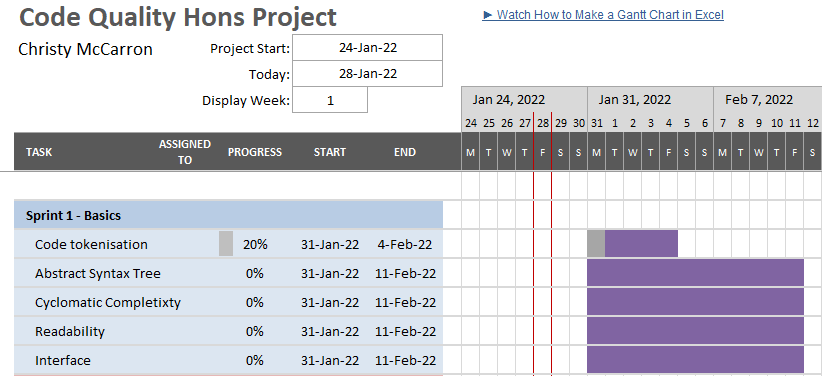
\includegraphics[width=.2\textwidth]{images/gantt.png}
    \caption{Gantt Sprint 1}
    \Description{gantt for sprint 1}
    \label{fig:gantt}
  \end{figure}
  Reflecting on the progress so far I believe that I have done a good amount of research which I will now apply to coding, I wish I had started prototying earlier as that would have made the planning much easier to estimate time.
  \newline
  As I am following agile I have made simple plans for sprint 1 where my sprints will be 2 weeks, after the end of sprint I will have a retrospective and review the progress completed in sprint 1.
  \newline
  I believe over the course of the project I should be able to complete every user story following this model.
  \newline
  The biggest pitfall that should be encountered is ensuring the abstract syntax tree is correct is this is the bed that everything else lies on, to ensure this it will be developed with a massive amount of unit and integration testing.